%!TEX root = ../main.tex

\chapter{Initial Results and Future Work}\label{cha:initial_results}
In this section the motivation of the methodology will be outlined and some initial results will be presented.
All code used was written in Python and used the Keras library \cite{chollet2015keras} with Tensorflow back-end \cite{tensorflow2015-whitepaper}.
Only very brief proof of concepts are shown, with some potential areas for future improvements outlined later.

\section{Method}\label{sec:method}
Autoencoders are a popular method in deep learning image analysis.
They consist of two parts, an encoder and a decoder which are often symmetrical.
The encoder takes in an image and compresses it to a lower resolution with more feature channels.
The decoder reconstructs the original image from the compressed version.
The neural network is trained to compress and reconstruct the image as accurately as possible.
Often this technique is used to find lower dimensional representations of images, possibly for feature extraction.
However, it can also be used for noise reduction and therefore cancer detection (we can think of a cancer hotspot as noise in a healthy image).

The process is as follows:

\begin{enumerate}
    \item Take a healthy (no cancer) image and add some random noise
    \item Train the autoencoder to reconstruct the original image that contains no noise
    \item When the autoencoder acts on an image containing cancer, it will treat the cancer as noise and remove it from the reconstruction.
    \item By comparing the reconstructed image and the original image, the cancer can be located easily.
\end{enumerate}

\subsection{Attempt 1}\label{subsec:attempt1}
This is the first attempt at creating an autoencoder to detect cancers.
It does not add any noise but merely compresses and rebuilds the image.
This autoencoder takes in a single slice, then (all layers are convolutional with kernel size 3x3) to encode the image:

\begin{itemize}
    \item Layer 1 - Produces 2 channels, activation is Relu, padding is Same
    \item Maxpooling (2x2)
    \item Layer 2 - Produces 4 channels, activation is Relu, padding is Same
    \item Maxpooling (2x2)
    \item Layer 3 - Produces 8 channels, activation is Relu, padding is Same
    \item Maxpooling (2x2) Gives the encoded representation.
\end{itemize}

To decode:
\begin{itemize}
    \item Upsampling
    \item Layer 4 - Produces 8 channels, activation is Relu, padding is Same
    \item Upsampling
    \item Layer 5 - Produces 4 channels, activation is Relu, padding is Same
    \item Upsampling
    \item Layer 6 - Produces 2 channels, activation is Relu, padding is Same
    \item Output - Produces 1 channels, activation is Sigmoid, padding is Same
\end{itemize}

The optimiser for the autencoder is AdaDelta and the loss is MSE.
The autencoder is trained only on negative slices that do not contain cancer and the results are shown in Figures \ref{fig:standard_neg} and \ref{fig:standard_pos}.

\begin{figure}[hbtp!]
    \centering
    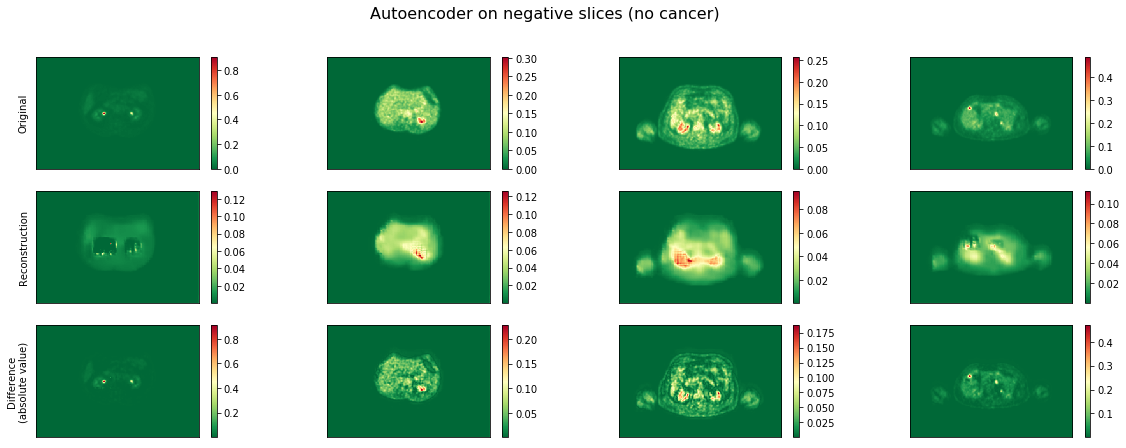
\includegraphics[width=\textwidth]{./img/standard_negative.png}
    \caption{Standard Autoencoder on Negative Slices (no cancer).}
    \label{fig:standard_neg}
\end{figure}

\begin{figure}[hbtp!]
    \centering
    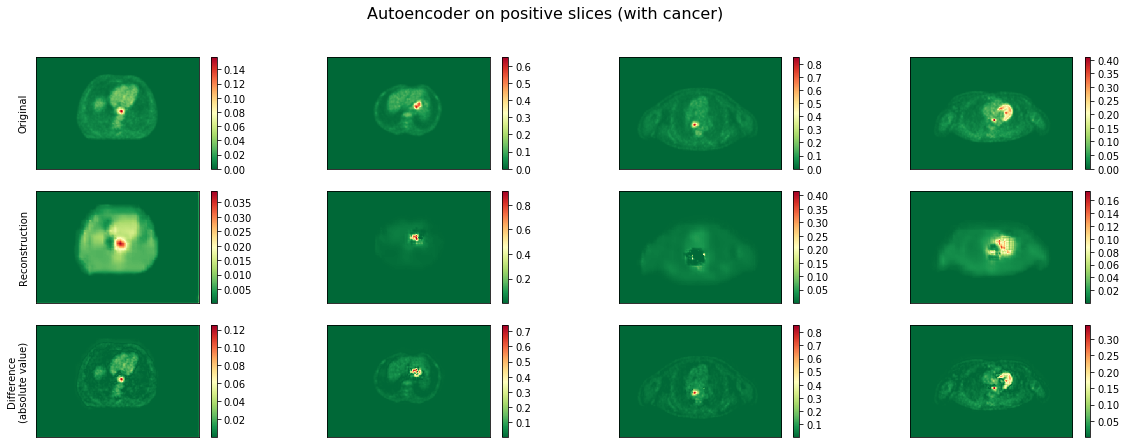
\includegraphics[width=\textwidth]{./img/standard_positive.png}
    \caption{Standard Autoencoder on Positive Slices (with cancer).}
    \label{fig:standard_pos}
\end{figure}

\subsection{Attempt 2}\label{subsec:attempt2}
The second attempt adds noise to the original image and is trained to remove it.
However, in this case there is no encoding or decoding step.
Again, the optimiser for the autencoder is AdaDelta and the loss is MSE.
The autencoder is trained only on negative slices and all layers are convolutional with kernel size 3x3:

\begin{itemize}
    \item Layer 1 - Produces 2 channels, activation is Relu, padding is Same
    \item Layer 2 - Produces 4 channels, activation is Relu, padding is Same
    \item Layer 3 - Produces 8 channels, activation is Relu, padding is Same
    \item Layer 4 - Produces 8 channels, activation is Relu, padding is Same
    \item Layer 5 - Produces 4 channels, activation is Relu, padding is Same
    \item Layer 6 - Produces 2 channels, activation is Relu, padding is Same
    \item Output - Produces 1 channels, activation is Sigmoid, padding is Same
\end{itemize}

The results for this attempt are shown in Figures \ref{fig:noisy_neg} and \ref{fig:noisy_pos}.

\begin{figure}[hbtp!]
    \centering
    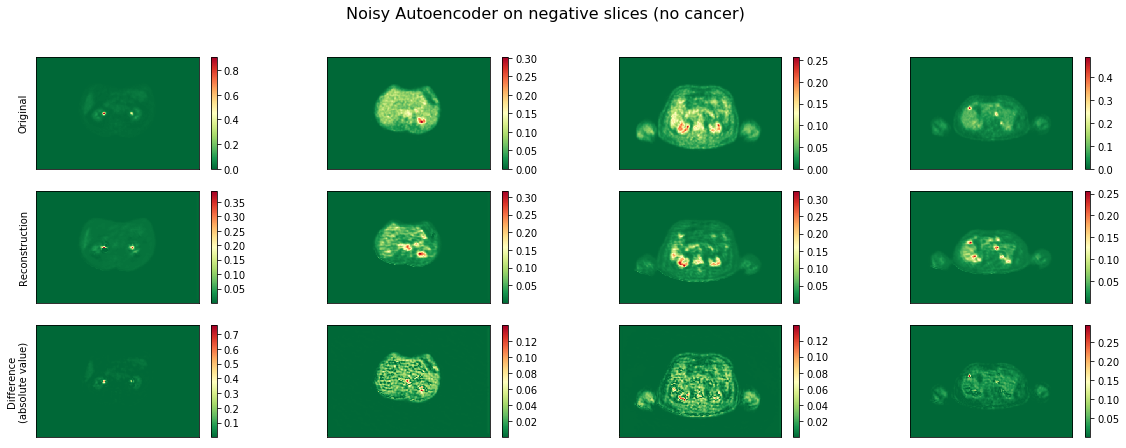
\includegraphics[width=\textwidth]{./img/noisy_negative.png}
    \caption{Noisy Autoencoder on Negative Slices (no cancer).}
    \label{fig:noisy_neg}
\end{figure}

\begin{figure}[hbtp!]
    \centering
    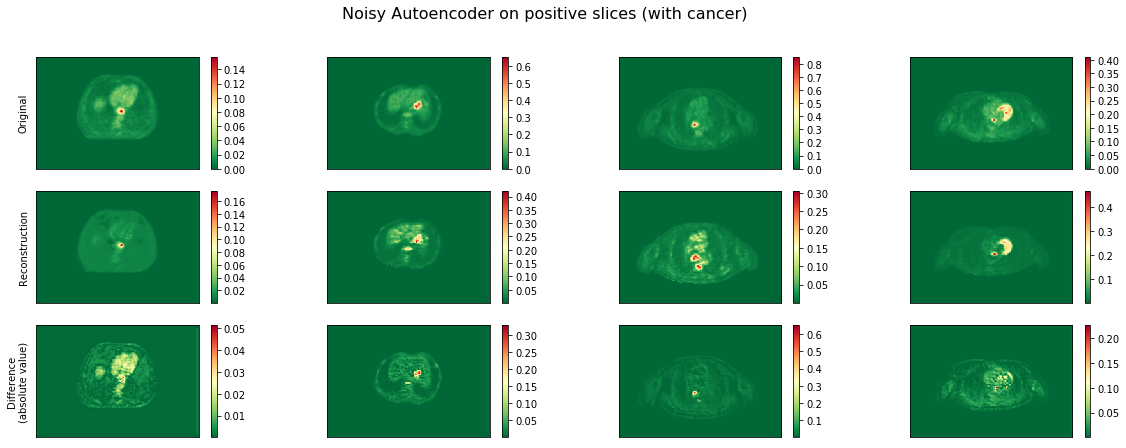
\includegraphics[width=\textwidth]{./img/noisy_positive.png}
    \caption{Noisy Autoencoder on Positive Slices (with cancer).}
    \label{fig:noisy_pos}
\end{figure}

\section{Results}
Both of the autoencoders outlined in Sections \ref{subsec:attempt1} and \ref{subsec:attempt2} are small proofs of concept.
Figures \ref{fig:standard_pos} and \ref{fig:noisy_pos} show images containing cancer for each of the autoencoders.
In the final row, the difference between the original image and the reconstruction is given.
It is clear that the addition of cancer is confusing the autoencoder such that in the reconstruction we have a hot-spot that stands out against the background more.
However, there isn't much of an improvement against the original image.

There are some possible reasons for this.
Firstly, the autoencoders may not be large enough.
Thus they don't have the capacity to remove noise and detect cancer.
Also, some slices that don't contain cancer still contain elements that glow brightly, for example the kidneys.
Therefore, the autoencoders will still learn to replicate hot-spots even though they are only trained on negative slices.

\section{Further Work}
There are many ways to extend this work and improve it.
Firstly, the two methods outlined in Sections \ref{subsec:attempt1} and \ref{subsec:attempt2} should be combined such that the autoencoder has an encoding part, a decoding part and is trained on noisy images.

Secondly, it should only be trained on slices with no brightly glowing sections.
This means any slices containing, cancer, kidneys or the brain should be removed.
By doing this, the autoencoder will only learn to reproduce healthy background information and will remove any noise/hot-spots.

Finally, it may be beneficial to replace Max Pooling steps with Average Pooling.
Max Pooling layers takes the maximum value of the pixels they are presented, thus maintaining information about high valued areas.
If they were replaced with Average Pooling layers, hot-spots wouldn't be transferred between layers and the autoencoder may find it easier to learn to remove them.

The robustness of the network should also be examined.
Adversarial networks have been successful in many areas involving natural images, but little work has been published with regards to medical images.
In order for deep learning to become accepted by medical practitioners, the risks and vulnerabilities needs to be better understood.

\section{Conclusion}
Deep learning for medical image analysis is a very powerful and common tool.
An overview of deep learning was given and much of the previous literature has been discussed.
So far this work has shown the the methodology outlined in Section \ref{sec:method} has the potential to locate cancers accurately, and some potential directions for future work have also been outlined.